\section{Advanced architecture development}
\graphicspath{{sec3/images/}}
In this section is analyzed the design of the same IIR filter seen previously but with an advanced architecture, developed with the J-look-ahead technique. The basic equation of the filter is the following:
$$ y[n] = b_0x[n] + b_1x[n-1] + a_1y[n-1]$$

The J-look-ahead technique involves rewriting the equation by replacing the term $y[n-1]$ by evaluating it as a function of $y[n-2]$.
$$ y[n-1] = b_0x[n-1] + b_1x[n-2] + a_1y[n-2]$$

Then it is possible to replace the result obtained in the starting equation:
$$ y[n] = b_0x[n] + b_1x[n-1] + a_1(b_0x[n-1] + b_1x[n-2] + a_1y[n-2])$$
$$ y[n] = b_0x[n] + (b_1 + a_1)x[n-1] + a_1b_1x[n-2] + {a_1}^{2}y[n-2]$$

While keeping the classical architecture of the IIR direct form II filter, the resulting equation can be implemented through the scheme of a second-order filter.

\begin{figure}[h]
	\center
	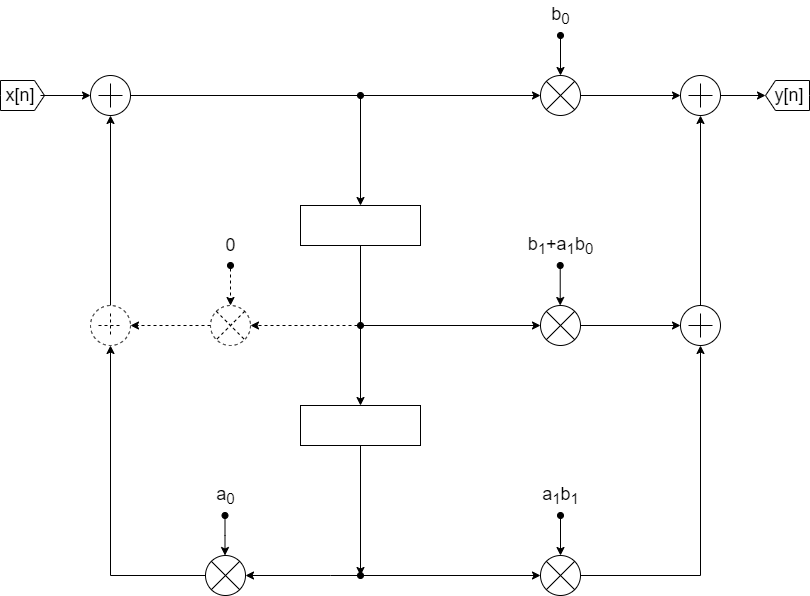
\includegraphics[width=0.65\textwidth]{IIR_2.png}
	\caption{IIR filter with J-look-ahead technique}
	\label{fig:IIR_advanced}
\end{figure}

\subsection{C model}

For the circuit, a C model was created for Fixed point analysis; for this model a new script written ad hoc was used, which uses a vector of 7 components to simulate the pipelined architecture of the component. The script name is \textit{J-look-ahead.c} and was included in the report delivery.The output signal from the filter was then analyzed on Matlab to evaluate its effectiveness. Then it was evaluated the Total Harmonic Distortion that, as you can observe from the \autoref{fig:THD_5_bit_IIR_JLA}, remained perfectly within the specifications.

\subsection{Design optimization}

This structure can be, as opposed to the previous version, improved in terms of performance. The critical path of this scheme consists of 4 combinatorial blocks, two multipliers and two adders, though by means of the appropriate transformations it is possible to reduce the longest combinatorial path.  In \autoref{fig:IIR_advanced_2} it has been identified the first cut-set that allows to move the register by changing the length of the critical path from 4 to 3.

\begin{figure}[htb]
	\center
	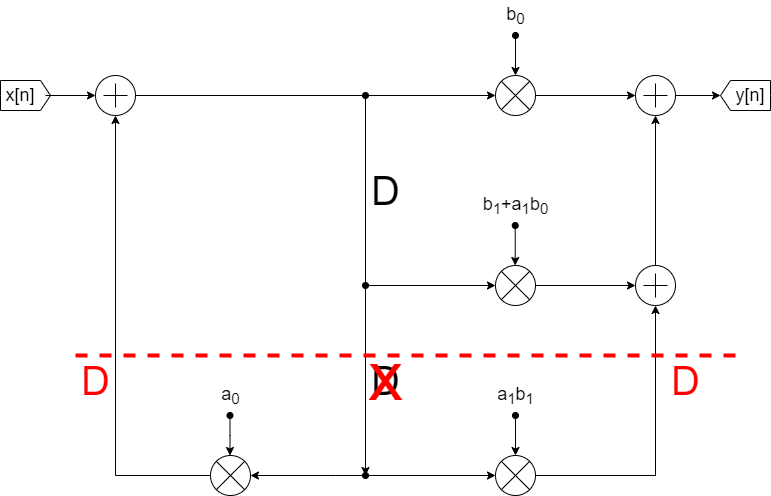
\includegraphics[width=0.55\textwidth]{IIR_2_1.png}
	\caption{Advanced architecture with $1^{st}$ transformation}
	\label{fig:IIR_advanced_2}
\end{figure}

In \autoref{fig:IIR_advanced_3} a feed-forward cut-set has been identified where it is possible to insert a pipeline stage on all three branches. In this way the combinatorial path including the $b_0$ multiplier is no longer part of the critical path. The longest combinatorial path includes the multiplier for the term $b_1 + a_1b_0$, the intermediate adder and the final adder. A further transformation allows to move the register from one side of the multiplier to the other without altering the behavior of the circuit, as in \autoref{fig:IIR_advanced_4}.

\begin{figure}[ht]
	\begin{minipage}[b]{0.5\linewidth}
		\centering
		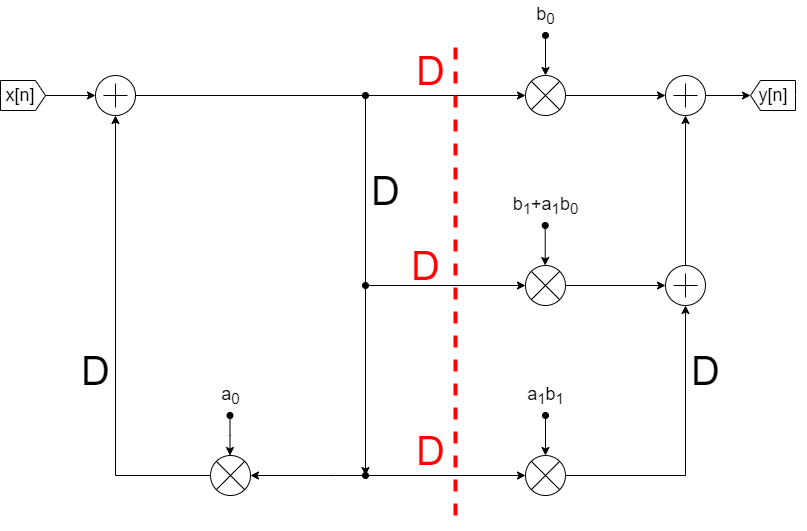
\includegraphics[width=\textwidth]{IIR_2_2.png}
		\caption{Advanced architecture with $2^{nd}$ transformation}
		\label{fig:IIR_advanced_3}
	\end{minipage}
	\hspace{0.5cm}
	\begin{minipage}[b]{0.5\linewidth}
		\centering
		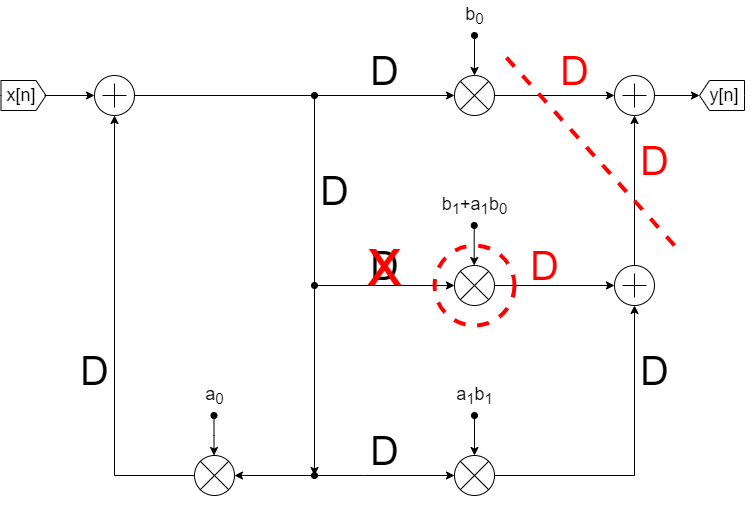
\includegraphics[width=\textwidth]{IIR_2_3.png}
		\caption{Advanced architecture with $3^{rd}$ transformation}
		\label{fig:IIR_advanced_4}
	\end{minipage}
\end{figure}

The latter transformation in \autoref{fig:IIR_advanced_4} takes into account the feed-forward cut-set on the two input branches at the last adder and through the insertion of a pipeline stage bring the critical path to be equal to the delay of a single multiplier.

In \autoref{fig:IIR_final} the optimized architecture of the IIR filter can be observed, in which a pipeline stage has been inserted between each combinatorial block. These transformations allow the circuit to reach the maximum throughput at the expense of latency, which compared to the initial circuit has increased from $2\,T_{ck}$ to $4\,T_{ck}$.

\begin{figure}[htb]
	\center
	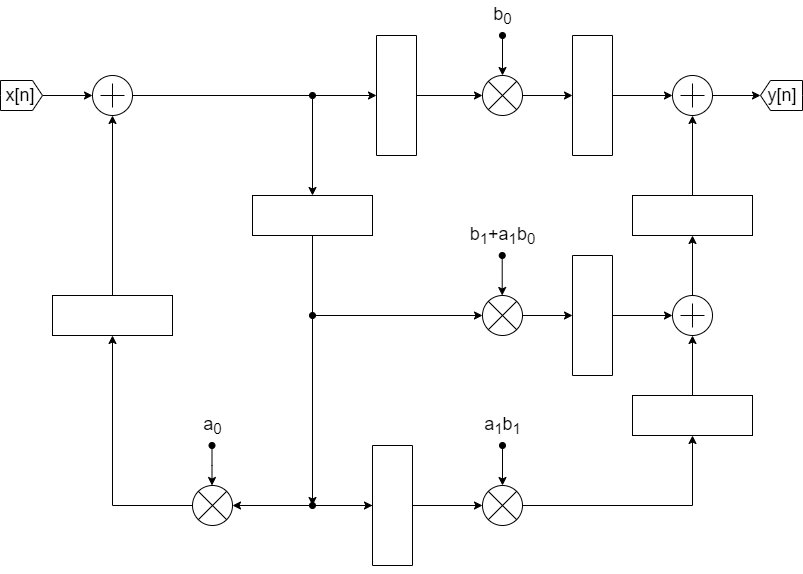
\includegraphics[width=0.65\textwidth]{IIR_final.png}
	\caption{Optimized architecture of J-look-ahead IIR filter}
	\label{fig:IIR_final}
	\end{figure}

\pagebreak
\subsection{C model}

For the circuit, a C model was created for Fixed point analysis; for this model a new script written ad hoc was used, which uses a vector of 7 components to simulate the pipelined architecture of the component. The script name is \textit{J-look-ahead.c} and was included in the report delivery.The output signal from the filter was then analyzed on Matlab to evaluate its effectiveness. Then it was evaluated the Total Harmonic Distortion that, as you can observe from the \autoref{fig:THD_5_bit_IIR_JLA}, remained perfectly within the specifications.

\subsection{Comparing Direct form II and J-Look-Ahead}
What will be presented now is an analysis of the data obtained from the two filters, with the aim of demonstrating their equivalence in behavior despite the great difference between the two topologies. In particular they will be examined in Matlab environment:

\begin{itemize}
	\item Initial signal values
	\item Average of the two signals
	\item Variance of the two signals
\end{itemize}

Notice that the IIR look-ahead filter topology in \autoref{fig:IIR_final} has two pipeline stages between the input and output signal, this implies that the signal has a higher latency than the Direct form II topology, which corresponds exactly to two clock cycles. The table in \autoref{fig:THD_table} shows the results of the two implementations.

\begin{figure}[ht]
	\begin{minipage}[b]{0.5\linewidth}
		\centering
		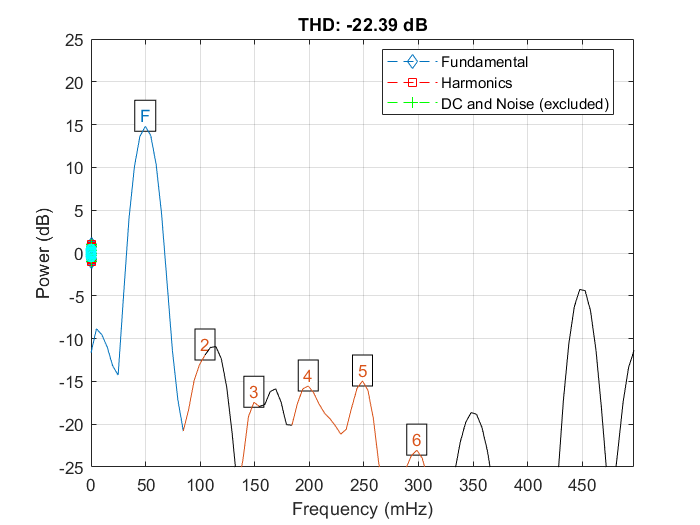
\includegraphics[width=\textwidth]{JLAH_THD_5_bit_C_result.png}
		\caption{THD of IIR J-Look-Ahead filter}
		\label{fig:THD_5_bit_IIR_JLA}
	\end{minipage}
	\hspace{0.5cm}
	\begin{minipage}[b]{0.4\linewidth}
		\centering
		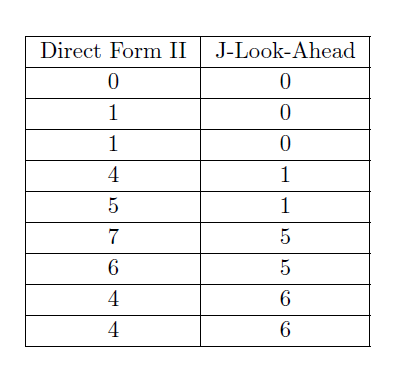
\includegraphics[width=\textwidth]{THD_table.png}
		\caption{Results of the two implementations compared}
		\label{fig:THD_table}
	\end{minipage}
\end{figure}

As the J-look-Ahead {THD} graph has anticipated, the two signals are not perfectly identical in the values and although the overall trend may be very similar, one may be interested in how different it actually is, so an analysis of the output signals from the two qualitative and quantitative filters is necessary at this point. Afterwards, the average and variance values of the two signals are represented:

\begin{table}[H]
	\begin{center}
		\begin{tabular}{|c|c|c|}
			\hline
			Parameter		& Direct Form II	& J-Look-Ahead 			\\ \hline
			Mean			&$-0.8308$  		& $-2.2537$	           	\\ \hline
			Variance		&$23.6312$      	& $32.9303$             \\ \hline
			
		\end{tabular}
	\end{center}
\end{table}

The two signals are not perfectly identical, and in fact they present different averages and variance, but they have the same order of magnitude and values consistent with the system under analysis. For a finer analysis it is necessary to use Allan's variance to measure how much the noise degrades the performance and how much the oscillatory behavior of the output is more or less stable. In \autoref{fig:Allan_Var} the variance of the two signals is represented and in \autoref{fig:Allan_Var_difference} the difference between the two variance to assess how much the stability of Direct Form II differs from that of J-Look-Ahead, both graphs were generated using the Matlab function \textit{allanvar()}:

\begin{figure}[ht]
	\centering
	\begin{minipage}[b]{0.44\linewidth}
		\centering
		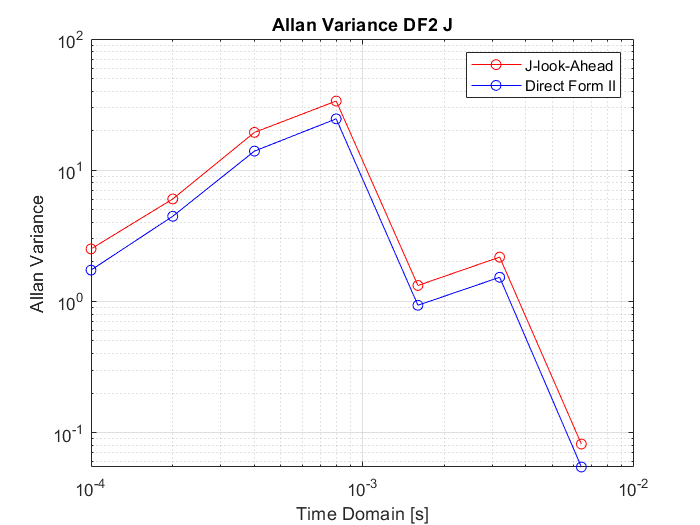
\includegraphics[width=\textwidth]{Allan Variance.png}
		\caption{Allan variance of the Direct Form II  and J-look-ahead IIR Filter}
		\label{fig:Allan_Var}
	\end{minipage}
	\hspace{0.5cm}
	\begin{minipage}[b]{0.48\linewidth}
		\centering
		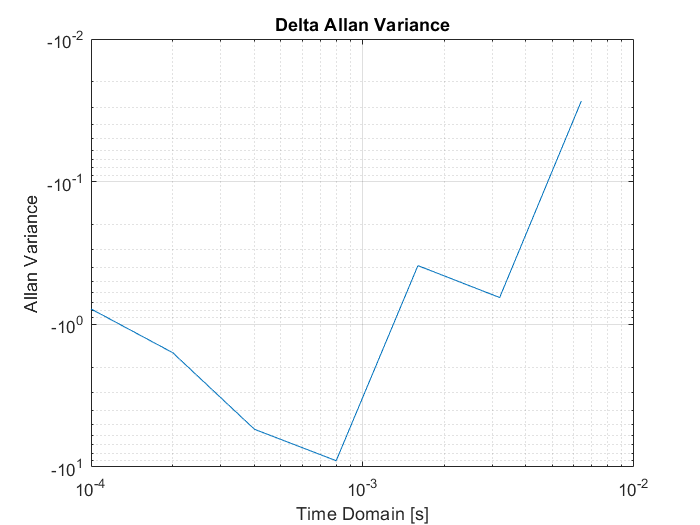
\includegraphics[width=\textwidth]{Allan Var difference.png}
		\caption{Difference of the 2 Allan variance}
		\label{fig:Allan_Var_difference}
	\end{minipage}
\end{figure}

\pagebreak
\subsection{Simulation}
For the simulation of the circuit has been used the same test-bench since the external entity of the circuit has not been modified with respect to the previous implementation.
In \autoref{fig:wave_start_j} the timing with the signals of the DUT is shown.In this case when the $VIN$ signal becomes valid 4 clock periods are required until the first result is available at the output; the explanation for this longer latency is due to the pipeline stages introduced in the circuit.

\begin{figure}[h]
	\center
	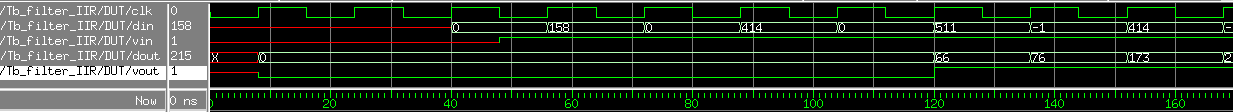
\includegraphics[width=1\textwidth]{wave_start_j_look_ahead.png}
	\caption{Start of the simulation}
	\label{fig:wave_start_j}
\end{figure}

Finally in \autoref{fig:wave_vin_j} it is observed the correct operation of the circuit when $VIN$ becomes low and then high. The internal registers do not sample when $VIN$ is not asserted, so the output data does not change, keeping the output valid. When $VIN$ returns to $1$, only one clock period is required before the output changes value because the registers are already full.

\begin{figure}[h]
	\center
	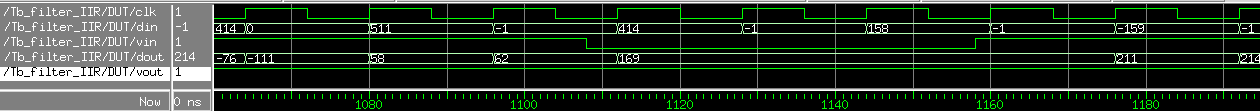
\includegraphics[width=1\textwidth]{wave_vin_0_1_j_look_ahead.png}
	\caption{Simulation of $VIN$ signal transition}
	\label{fig:wave_vin_j}
\end{figure}

Once the correct timing of the circuit has been verified, the output data has been compared with the corresponding C implementation of the realized model. With the same set of data used for the test-bench of the previous architecture, the same output results were obtained. You can refer to the data shown in \autoref{tab:tab_results} to have an outline of the results.
\subsection{Logic Synthesis}
The synthesis of the circuit was done with the Synopsys software. The first objective is to determine the maximum frequency that will allow the correct operation of the circuit and its area. The standard port libraries provided have been used to automatically synthesize even the complex logical blocks such as adders and multipliers.
In a preliminary phase a clock with period $T_{clk} = \SI{10}{\nano\second} \pm \SI{0.07}{\nano\second}$ has been set. The result of the synthesis shows a slack of $+\SI{5.14}{\nano\second}$; the fact that the slack is positive implies that the clock constraints set have been met with the synthesis obtained.
To evaluate the maximum operating frequency of the circuit, a clock period of 0 has been set, so theoretically the negative slack obtained should correspond to the minimum necessary clock period. However, this is only partially true, since setting the clock period to the new value will still result in a negative slack. This behavior is due to the fact that the synthesizer changes the structure of the internal slack according to the constraint provided on the clock as you can see from the data on the area. It was necessary to iterate this procedure several times to obtain a slack equal to 0 and therefore the maximum operating frequency of the circuit. In \autoref{tab:timing_rep} a summary of the results obtained is shown.

\begin{table}[h]
\begin{center}
\begin{tabular}{|l|l|l|}
\hline
$T_{CLK}$ (ns) & slack (ns) & area $(\SI{}{\micro\meter})^2$ \\
\hline
10 & 5.14 & 1991 \\
0 & -3.13 & 2491 \\
4.10 & 0 & 2187 \\
16.4 & 11.54 & 1991 \\
\hline
\end{tabular}
\end{center}
\caption{Results of timing report}
\label{tab:timing_rep}
\end{table}

The second goal is to find area and power consumption by setting $T_{CLK} = 4 T_{min}$. For the area you can refer to \autoref{tab:timing_rep}. For the power computation, a record of the switching activity has been generated through a Modelsim simulation and saved on a vcd file, subsequently converted in saif file. The presence of these data serves during the calculation of the correct power consumption in the Synopsys environment. The results are shown in \autoref{fig:pow_rep_x4}.

\begin{figure}[htb!]
	\center
	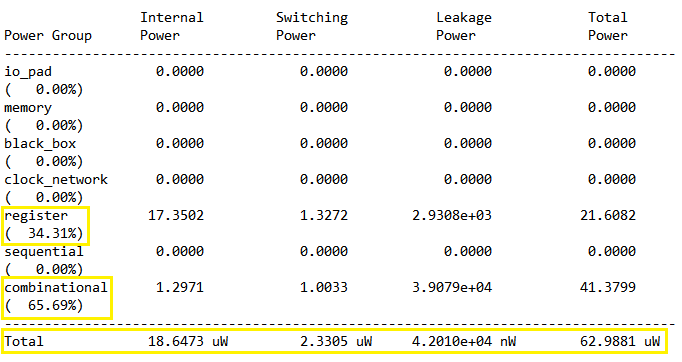
\includegraphics[width=0.8\textwidth]{rep_power_x4_mod.png}
	\caption{Power Report}
	\label{fig:pow_rep_x4}
\end{figure}

It can be seen that the power is divided between the registers and the combinatorial part with a preponderance of this second contribution, $65\%$, due to the presence of 3 multipliers and 2 adders in the designed architecture.

\subsection{Place \& Route}
The last operation is the place and route of the circuit using the Innovus software. The netlist generated by Synopsys with $T_{CLK} = 4 T_{min}$ and the standard libraries have been used as a starting point. After the various required steps the final circuit shown in \autoref{fig:layout} has been obtained.

\begin{figure}[htb]
	\center
	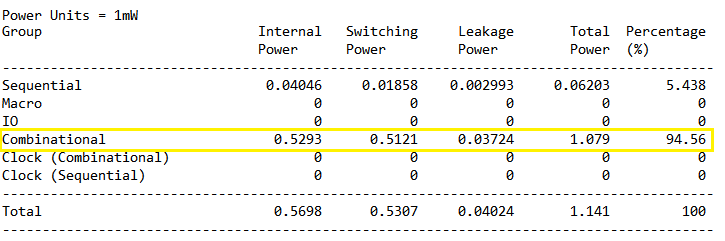
\includegraphics[width=0.7\textwidth]{rep_power_x4_cadence_mod.png}
	\caption{Post place \& route power report}
	\label{fig:cadence_pow_rep_x4}
\end{figure}

\begin{figure}[htb!]
	\center
	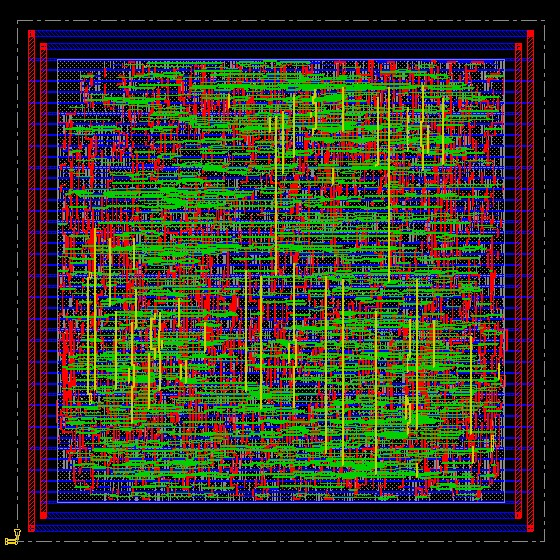
\includegraphics[width=0.5\textwidth]{IIR_filter_period_min_x4_place.jpg}
	\caption{Resulting layout}
	\label{fig:layout}
\end{figure}

The product layout has an area of $\SI{1959}{\micro\meter}^2$, which is in agreement with the estimated Synopsys' estimate shown in \autoref{tab:timing_rep}, with a total of 986 cells and 2455 gates. Then the timing analysis was launched to verify that the timing constraints were correct, then the connectivity and geometry was verified. Finally, using the switching activity calculated with Modelsim, the power consumption has been re-estimated. The results obtained are shown in \autoref{fig:cadence_pow_rep_x4}.


The power values obtained are in agreement with those obtained by Synopsys in \autoref{fig:pow_rep_x4}. Moreover, since the calculation at this level is much more accurate as it takes into account the physical layout of the circuit, it can be seen that in fact the consumption of the combinatorial part is prevalent.

